\interlude[1]{Hybridization}
\begin{frame}[light,s]{}
  \vspace{1cm}
  \large
  \vollkorn

  \begin{columns}[c]
    \begin{column}{.30\linewidth}
      % \vfill
      %  …that hybrid, practical, post-quantum cryptography is built by combining pre-quantum and post-quantum primitives.

      % \vfill
      %  …that key encapsulation methods can be combined, rendering a protocol like Rosenpass useful in pre-quantum as well
      %  as post-quantum settings.

      %  \vfill
      %  …why combining protocols like WireGuard and Rosenpass directly is still useful to enable code-reuse and to avoid
      %  loosing trust in established systems like WireGuard.
      %  \vfill
      In the following slides you will learn…
      \par\vspace{1.5em}
      …that hybrid security can be achieved by building hybrid primitives and that it is not always wise to do so.
    \end{column}

    \begin{column}{.40\linewidth}
      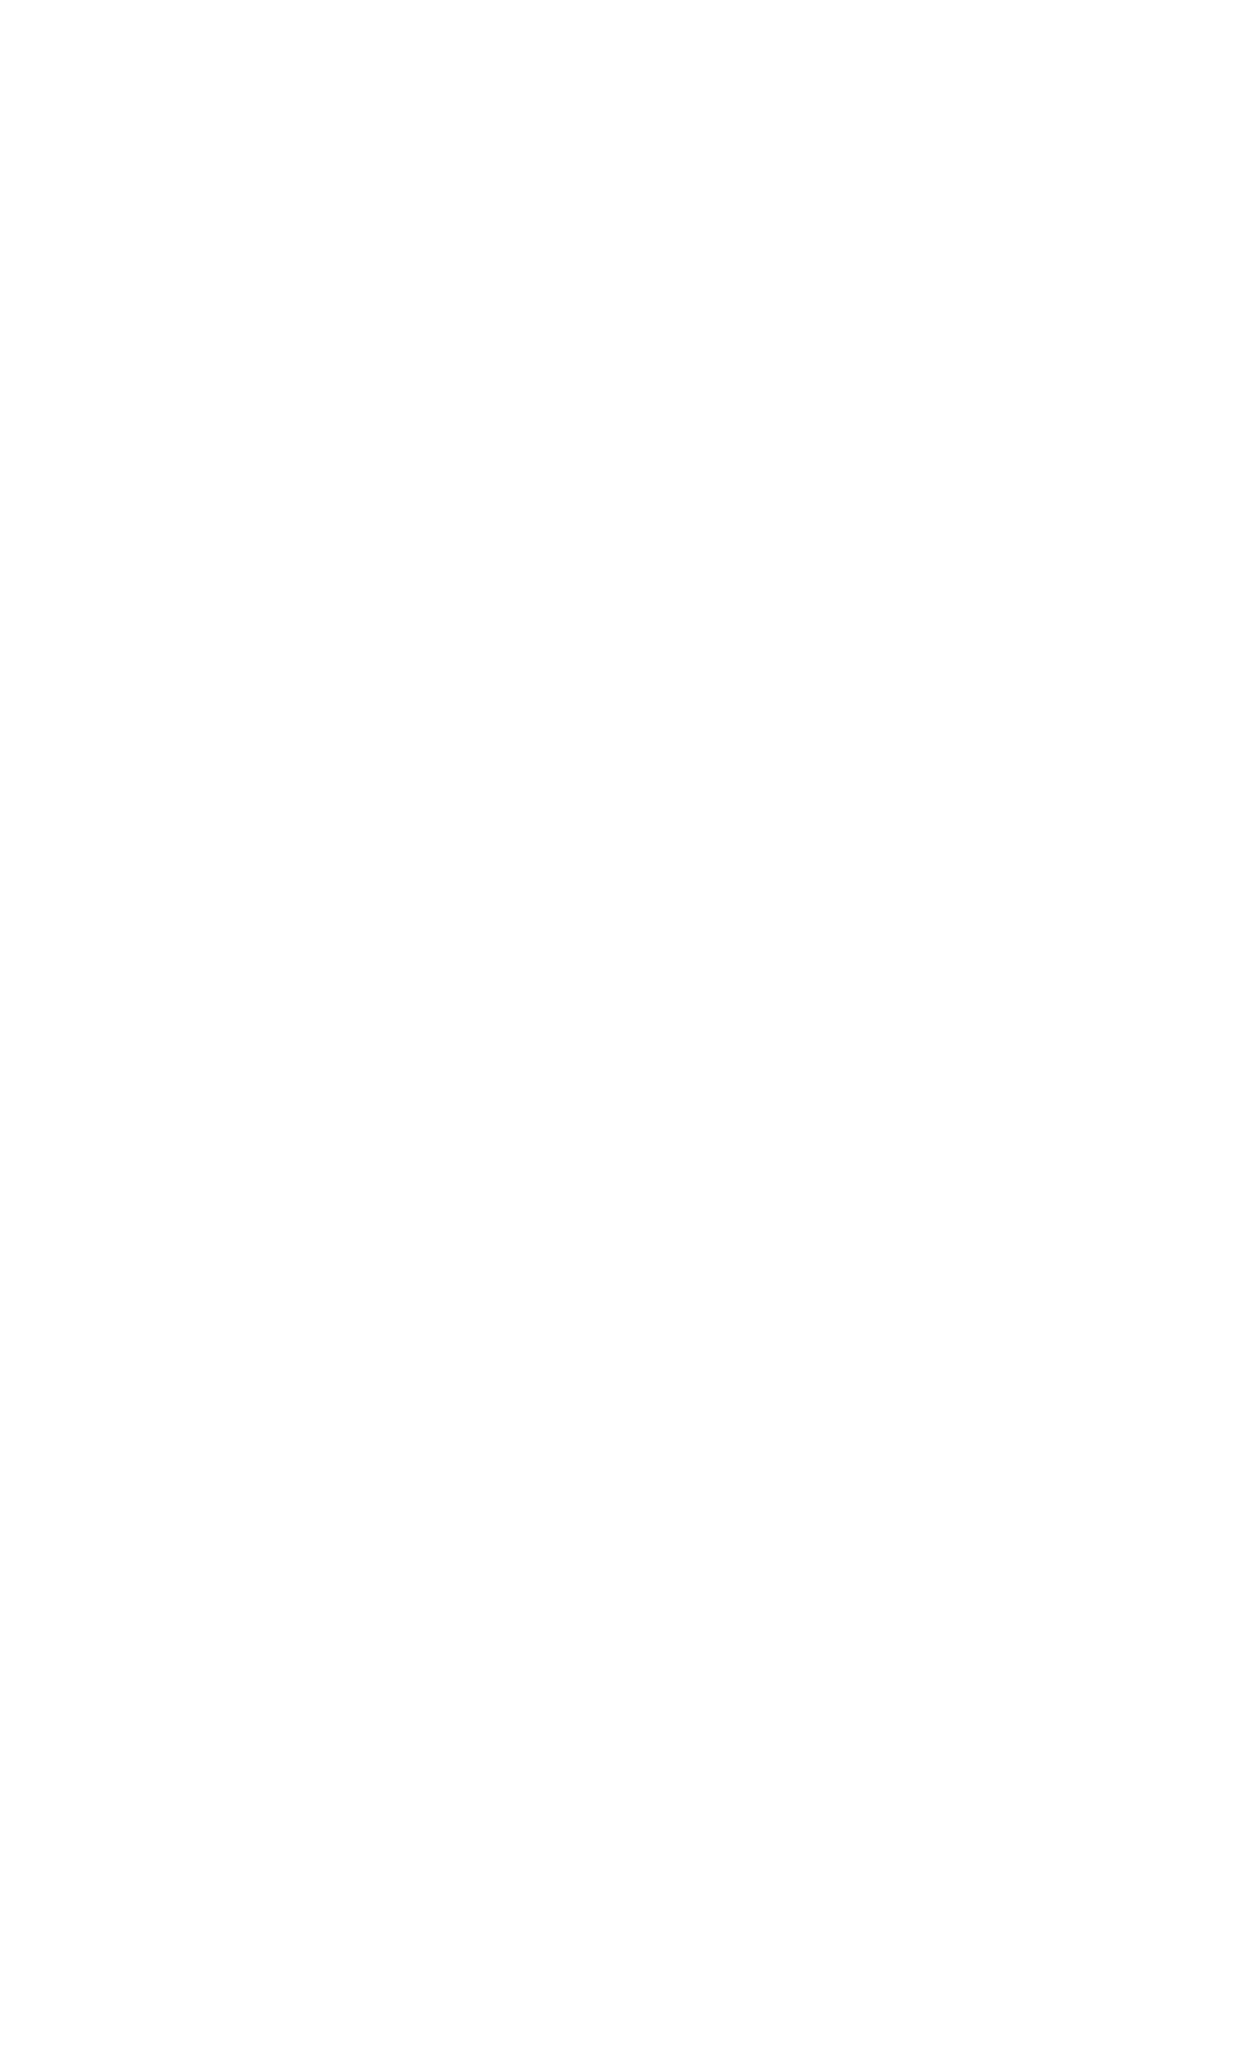
\includegraphics[width=.7\linewidth,padding=-.2cm .2cm .2cm .2cm]{graphics/krapfen-prezel-bunny.pdf}
    \end{column}
  \end{columns}
\end{frame}

\begin{frame}{Combining two KEMs with the GHP-Combiner}
  \centering
  \includegraphics[height=.92\textheight,page=1,clip=true,trim={0.5cm 1cm 0.7cm 1.5cm}]{graphics/rosenpass-encapsulation-combiner.pdf}
\end{frame}

\begin{frame}{Turning a NIKE into a KEM}
  \centering
  \includegraphics[height=.92\textheight,page=2,clip=true,trim={0.5cm 1cm 0.7cm 1.5cm}]{graphics/rosenpass-encapsulation-combiner.pdf}
\end{frame}

\begin{frame}{X-Wing}
  \centering
  \includegraphics[height=.92\textheight,page=3,clip=true,trim={0.5cm 1cm 0.7cm 1.5cm}]{graphics/rosenpass-encapsulation-combiner.pdf}
\end{frame}

\begin{frame}{Rosenpass \& WireGuard Hybridization}
  \centering
  \includegraphics[height=1.03\textheight, clip=true,trim=0cm 0cm 0cm 3.2cm]{graphics/rosenpass-wireguard-hybrid-security.pdf}
\end{frame}
